\section{Methodology}
\label{sec:methodology}

This section describes how the gaps identified in
Section~\ref{sec:relatedwork} are translated into a concrete
artefact: a challenge web-exploitation suite with a
shared personalisation layer, reproducible containerisation,
and an end-to-end testing regime whose outputs form the
evidence base for Section~\ref{sec:results}.

\subsection{Design Philosophy}
\label{sec:design-philosophy}

Five principles were established at the outset and applied
uniformly across the suite. \textit{Realism over
artificiality}: every challenge is scenario-wrapped as an
application a student could plausibly encounter (a password manager, an HR system, etc...), so that
exploitation exercises the path to the flag rather than a
synthetic puzzle~\cite{Fuzyll2015,Vykopal}.
\textit{Within-domain scaffolding}: stages inside a challenge
gate each other through in-application breadcrumbs
(\texttt{CHANGELOG} entries, \texttt{/health} metadata, the
visible source of a WAF) rather than through external hints,
maintaining challenge and skill balance across the cohort's
skill distribution~\cite{Csikszentmihalyi,Balaji2025}.
\textit{Broad OWASP coverage}: the suite deliberately includes
modern classes (such as SSTI, SSRF, and insecure deserialisation) that
Sasiwanit et al.~\cite{Sasiwanit} identify as under-represented
in existing platforms. \textit{Per-user integrity}: flags are
derived deterministically from a per-deployment secret salt
and embed the recipient's username, making sharing both
attributable and invariant across cohorts
(Section~\ref{sec:flag-personalisation}). \textit{Stack
diversity}: challenges vary by primary
technology stack (with a preference for more common modern tech stack and frameworks), forcing the player to adapt to different
framework idioms rather than pattern-matching a single stack.

\subsection{Suite Architecture}
\label{sec:challenge-architecture}

Table~\ref{tab:suite-summary} summarises the challenges
and their OWASP coverage. The suite is designed in a
jeopardy format: challenges are independent of one another
and can be attempted in any order, with each challenge
carrying a point value proportional to its flag count and
difficulty tier. A student might begin with a single-step
cookie manipulation in CTF1 and later attempt a four-stage
SSRF chain in CTF6, or tackle them in reverse; the
progressive difficulty described in
Section~\ref{sec:design-philosophy} provides a recommended
trajectory but does not impose a mandatory sequence.
Collectively, six of the ten 2021 OWASP categories are
represented, and the injection category (A03) is further
decomposed into SQL injection (CTF3), DOM-based XSS (CTF4),
and server-side template injection (CTF5). The four omitted
categories either resist flag-ification (A04 Insecure
Design, A09 Logging and Monitoring Failures), would require
shipping genuinely vulnerable dependencies into the
distributable (A06), or concern CI/CD rather than the web
layer (A08).

\begin{table*}[t]
\centering
\caption{Challenge Suite Summary}
\label{tab:suite-summary}
\begin{tabular}{|c|p{2.4cm}|p{3.6cm}|p{1.4cm}|p{3.0cm}|c|c|}
\hline
\textbf{CTF} & \textbf{Scenario} & \textbf{Vulnerability Classes} & \textbf{OWASP} & \textbf{Stack} & \textbf{Flags} & \textbf{Tier} \\ \hline
1 & Module portal &
Unsigned session cookie; privilege escalation &
A01, A02 &
Node.js, Express, EJS & 1 & Basic \\ \hline
2 & Password manager &
Weak JWT secret via PoW; JWT forgery &
A02, A07 &
Node.js, React/Vite, JWT & 1 & Basic \\ \hline
3 & Corporate HR system &
SQL injection (filter bypass); AES-CBC decryption; info disclosure &
A02, A03, A05 &
PHP/Laravel, React, PostgreSQL & 4 & Intermediate \\ \hline
4 & Corporate helpdesk &
DOM XSS (\texttt{eval}); bot-based escalation &
A03, A07 &
Node.js, React, PostgreSQL, Redis, BullMQ, Playwright & 1 & Intermediate \\ \hline
5 & NovaCMS blog/CMS &
SSTI (Jinja2); WAF bypass; RCE via MRO chain &
A01, A03, A05 &
Python/Flask, Jinja2 & 4 & Advanced \\ \hline
6 & Veridian Secure &
SSRF; IMDSv1 enumeration; Redis pivot (\texttt{dict://}) &
A10, A05, A01 &
Rust/Actix-web, Redis, simulated IMDS & 4 & Advanced \\ \hline
7 & NorthSide Notes &
Insecure deserialisation (CVE-2017-5941) &
A08 &
Node.js, Express, EJS, \texttt{node-serialize} & 1 & Basic/Intermediate \\ \hline
\end{tabular}
\end{table*}

\begin{figure}[t]
    \centering
    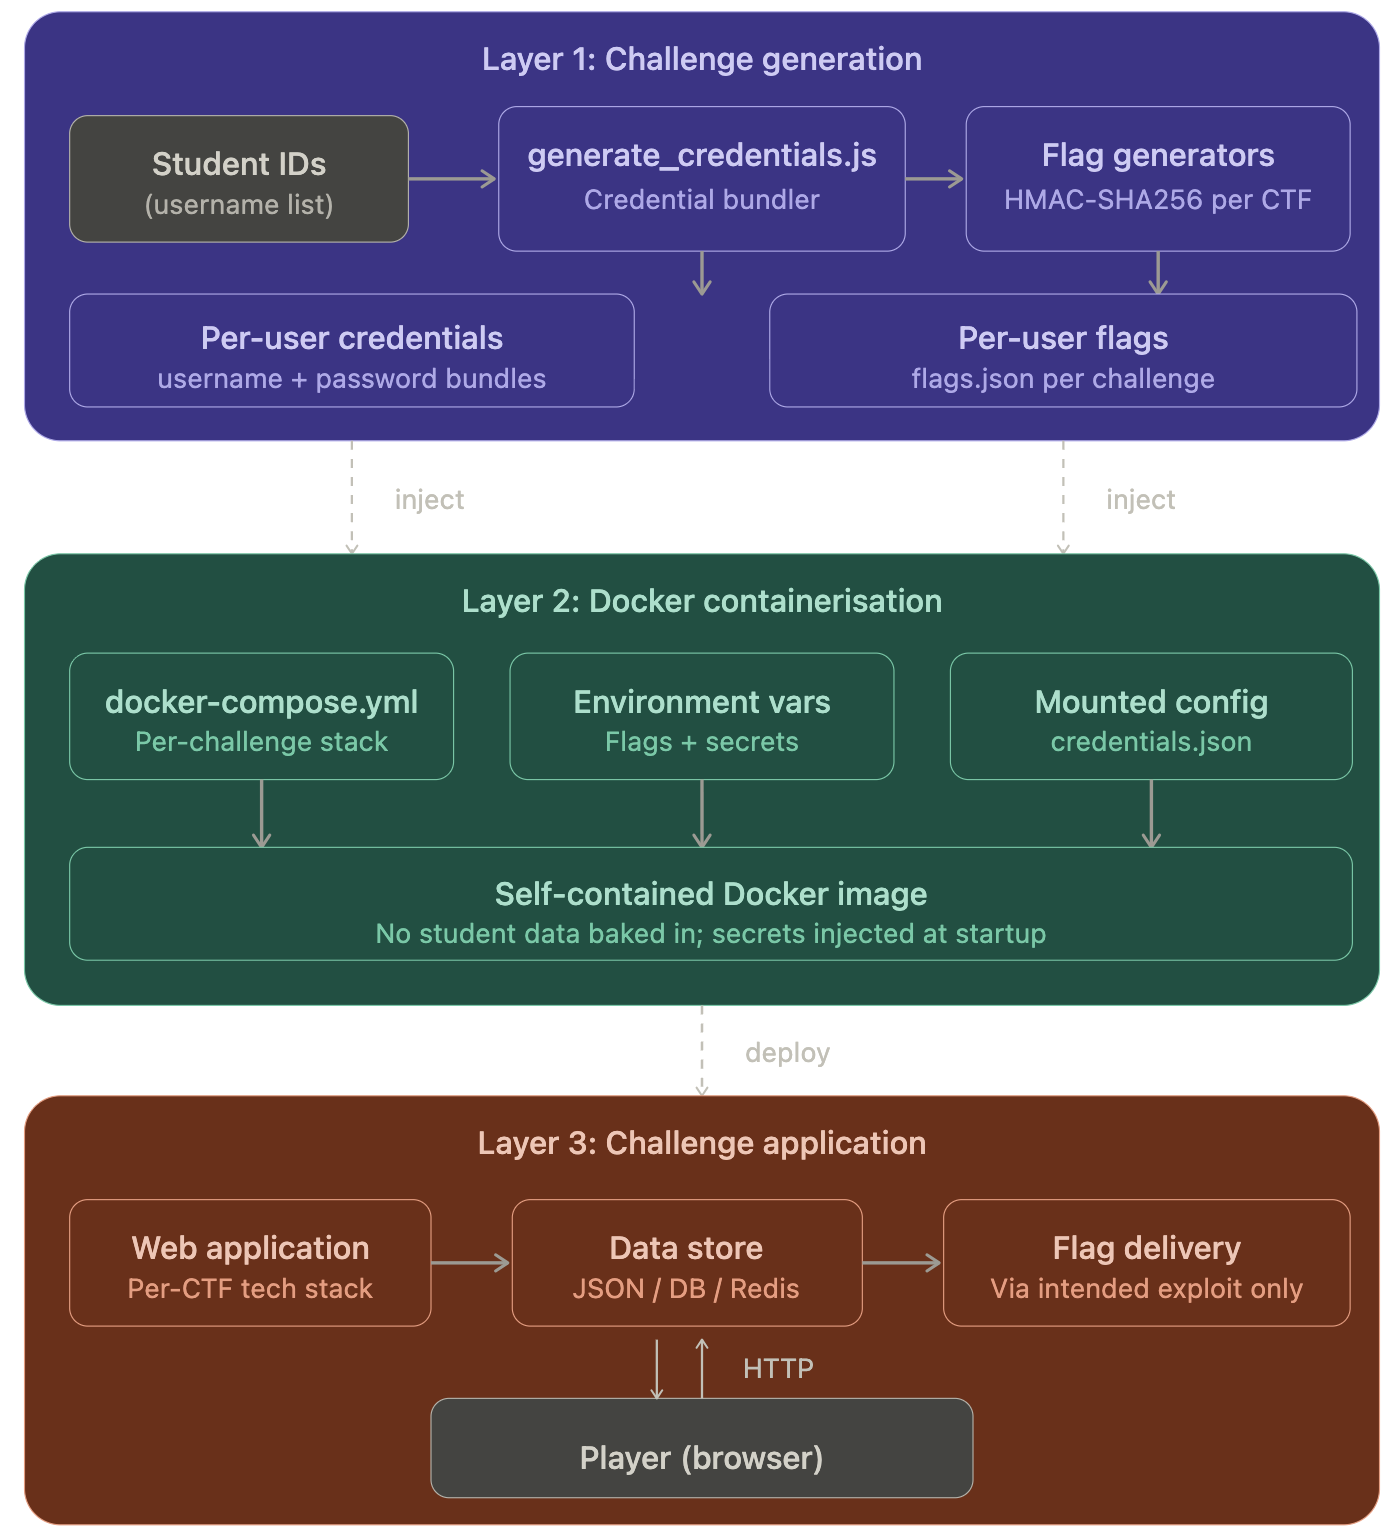
\includegraphics[width=\columnwidth]{figures/ctf_shared_infrastructure_architecture.png}
    \caption{Three-layer shared infrastructure: a generation
    layer produces per-user flags and credentials; a
    containerisation layer packages each challenge as a Docker
    Compose stack; and a challenge application layer
    implements the vulnerable behaviour. Generated by
    Anthropic Claude (2026)~\cite{ClaudeDiagram2026}.}
    \label{fig:architecture}
\end{figure}

All challenges share the three-layer architecture shown in
Figure~\ref{fig:architecture}. The \textbf{generation layer}
(Section~\ref{sec:flag-personalisation}) produces per-user
flags and credentials; the \textbf{containerisation layer}
(Section~\ref{sec:containerisation}) packages each challenge
with no student data baked into the image; and the
\textbf{challenge application layer}
(Section~\ref{sec:challenge-design}) implements the vulnerable
behaviour. The layers are decoupled so that a new cohort is
onboarded by re-running the generation scripts alone, without
any modification to challenge source or container images.

\subsection{Per-User Flag Personalisation}
\label{sec:flag-personalisation}

\subsubsection{Threat Model}

The existing Networks and Systems VM distributes an identical
image with statically randomised flags. This admits three
integrity threats: \textit{solution sharing} (a working
exploit is communicated verbatim to the cohort);
\textit{flag copying} (per-VM flags obtained via messaging or
screenshots are resubmitted); and \textit{LLM-assisted
solving} (uniform problem structures resembling public
write-ups are trivially solved by a prompted
model~\cite{ji2025}). The scheme described below addresses
flag copying and LLM-assisted solving directly. Solution
sharing is addressed structurally through multi-stage chain
design: a four-stage chain cannot be communicated as a single
payload and still requires the receiver to execute each stage
against their own instance.

The existing module's flag generation framework provides a
class-based, template-driven pipeline designed to produce
per-student zip packages for VM or server deployment. Because
the challenges in this project are distributed as Docker
Compose stacks rather than provisioned VMs, and because each
challenge uses a different technology stack with its own data
ingestion format, the templating and server-deploy
infrastructure of the upstream framework was unnecessary
overhead. A purpose-built replacement was therefore
implemented: lightweight standalone scripts that invoke
pluggable per-challenge generator modules and write
\texttt{flags.json} and \texttt{credentials.json} directly
into each challenge's data directory. The core cryptographic
primitive is unchanged (HMAC-SHA256 keyed on a deployment
salt), but the surrounding machinery is reduced from a
class hierarchy with template expansion and remote deployment
to a single-command invocation per challenge, better suited
to the container-native distribution model adopted by this
project.

\subsubsection{HMAC-SHA256 Flag Derivation}

Six of the seven challenges derive flags deterministically
from a per-deployment salt $s$ and a student username $u$ via
HMAC-SHA256~\cite{rfc2104}:
\begin{equation}
\mathit{token} = \mathrm{HMAC\text{-}SHA256}(s, u).\mathit{hex}[{:}N]
\label{eq:hmac-flag}
\end{equation}
\begin{equation}
\mathit{flag} = \mathit{prefix}\texttt{\{}\mathit{token}\texttt{\_}u\texttt{\}}
\label{eq:flag-format}
\end{equation}
where $N$ is the token length in hexadecimal characters
(16 for Basic-tier single-flag challenges and 20 elsewhere,
corresponding to 64- and 80-bit entropy respectively). For
example, with prefix \texttt{durham}, salt
\texttt{basic1-default-salt}, and username \texttt{abcd12},
the generator produces
\texttt{durham\{3a1f9c2b4e7d8a0f\_abcd12\}}. HMAC-SHA256 was
selected for three properties. \textit{Determinism}: $(s, u)$
always yields the same token, so flags can be regenerated
from the student roster alone without persistent state.
\textit{Collision resistance}: the 64-bit birthday bound is
approximately $2^{-32}$ for cohorts of
100--200~\cite{HMACNIST}. \textit{Deployment isolation}:
changing $s$ produces a disjoint flag space, so flags or
write-ups from a previous cohort are invalid without any
source-code change.

Multi-flag challenges (such as CTF3) derive per-flag
salts from a base salt by concatenation:
\begin{equation}
s_i = \mathit{base\_salt}\texttt{-flag}i, \quad i \in \{1, \dots, 4\}
\label{eq:per-flag-salt}
\end{equation}
Because HMAC-SHA256 under distinct keys produces
statistically independent outputs, capturing one flag reveals
no information about any other flag for the same user.

\subsubsection{Integrity Properties and Positioning}

Three properties follow directly from
equations~(\ref{eq:hmac-flag})--(\ref{eq:per-flag-salt}).
\textbf{Attribution}: because $u$ is embedded in the flag
string, any submitted flag identifies its legitimate owner;
submitting another student's flag is detectable without
server-side comparison. \textbf{Year-over-year invalidation}:
rotating $s$ invalidates all previously generated flags,
including any published write-ups. \textbf{LLM resistance}:
because $s$ is never exposed on the user-facing surface, an
LLM without the salt cannot produce a valid flag even when it
has correctly identified the methodology; the model may still
guide the student, but the flag itself must be produced by
executing the exploit against the student's personalised
instance. These claims are evaluated empirically in
Section~\ref{sec:results}.

The scheme is scoped deliberately to the flag layer. Chothia
and Novakovic's SecGen~\cite{chothia2023} randomises the
entire lab environment per student, defending against both
flag copying and methodology sharing.
Reimplementing SecGen-style environment generation across
seven distinct technology stacks would have required
infrastructure investment disproportionate to the target
context, and flag-layer personalisation captures the dominant
integrity risk (exam-style flag sharing) at a fraction of the
cost.

\subsection{Challenge Implementations}
\label{sec:challenge-design}

Full per-challenge documentation is available in the
submission's source tree; this section concentrates on the
four design decisions that constitute the principal novelty
of the suite, each of which operationalises one of the
guiding principles of
Section~\ref{sec:design-philosophy}.

\textbf{Accepting multiple cookie encodings (CTF1).} The
unsigned-cookie challenge's decoder accepts raw JSON, base64,
URL-encoded base64, and URL-encoded JSON. This is a
deliberate pedagogical choice: pilot attempts revealed that
players who correctly identified the vulnerability
frequently failed to exploit it because the browser had
URL-encoded the cookie on re-submission through DevTools.
Accepting multiple encodings keeps the vulnerability's
\textit{concept} as the barrier and removes an incidental
formatting trap, consistent with Fuzyll's maxim that
learning should be the path to the
flag~\cite{Fuzyll2015}. Post-design auditing also identified
an unintended login-bypass path (the form accepted the
base64 admin cookie as a password) which was removed; a
sliding-window per-IP rate limiter now forces the player
onto the intended cookie-tampering path.

\textbf{Disclosing the WAF source to the player (CTF5).} The
Jinja2 SSTI challenge in NovaCMS is gated by a twelve-word
keyword blocklist whose full source is served as a static
\texttt{CHANGELOG.md} asset advertised in the editor. The
challenge is therefore not ``guess the blocklist'' but
``reason about how to bypass a blocklist you can read,''
shifting the learning outcome from enumeration to
construction: players apply hex-escaped
\texttt{\textbackslash x5f\textbackslash x5f} dunders and the
Jinja \texttt{|attr()} filter to traverse the engine's MRO
chain from \texttt{lipsum} to \texttt{os.environ} where the
flag lives~\cite{JinjaMRO}. Because the WAF is visible, the
challenge admits a calibrable difficulty surface: raising the
bar is a matter of adding blocked substrings rather than
obfuscating the filter.

\textbf{Rewriting the IMDS link-local address (CTF6).}
Docker's default bridge network does not route the AWS
link-local metadata address \texttt{169.254.169.254}, yet
teaching a Capital One-style SSRF-to-IMDS
chain~\cite{khan2022} requires the player to supply exactly
that address. The Rust preview handler therefore rewrites
\texttt{169.254.169.254} to the Compose service hostname
\texttt{metadata} before dispatching the request, so the
player's mental model matches the real cloud environment
while the container network actually delivers the traffic.
The same handler supports \texttt{dict://} and
\texttt{gopher://}, which enables the Redis pivot documented
by PortSwigger~\cite{BurpSSRFRedis} and generalises the
lesson beyond the single IMDS surface.

\textbf{Per-student attribution via a file path (CTF7).} The
insecure-deserialisation challenge exposes each flag as a
per-user text file at
\texttt{/app/src/data/flag-files/<u>.txt}. The intended
payload, an immediately-invoked function expression passed to
\texttt{node-serialize}'s
\texttt{unserialize()}~\cite{CVE20175941,NodeSerialize}, must
embed the student's own username in the path to retrieve the
flag: any attempt to read another student's flag names the
target explicitly, so the exploit itself constitutes
attributable evidence of attempted impersonation,
complementing the embedded-username attribution of
equation~(\ref{eq:flag-format}).

Two further challenges warrant brief mention. CTF2 hides the
JWT signing secret behind a four-byte Proof-of-Work gate on a
debug endpoint, modelling the real-world pattern in which a
debug surface is ``protected'' by an obscure filter rather
than by authentication; the player then forges a JWT against
a \texttt{flag12} account whose vault entry is synchronised
from \texttt{flags.json} at startup. CTF3 includes a
deliberate alternative path
(\texttt{/api/debug/user-config} annotated
\texttt{// TODO: REMOVE BEFORE PRODUCTION}) that bypasses the
SQL-injection stage; both paths are pedagogically valid, and
the SQL path is rewarded through a second flag that the
debug path does not unlock.

\subsection{Containerisation and Distribution}
\label{sec:containerisation}

Each challenge is packaged as a Docker Compose
stack~\cite{DockerDocs}. Three constraints derived from the
threat model shape the packaging.
\textit{No student data in the image}: flags and credentials
are supplied as read-only bind mounts at startup
(\texttt{./flags.json:/app/flags.json:ro}), so rotating a
cohort is a matter of replacing the host-side files and
restarting the stack rather than rebuilding.
\textit{No code-change onboarding}: the generation layer
writes to the mount point only, leaving the image untouched.
\textit{No incidental exposure}: the simulated IMDS and the
unauthenticated Redis in CTF6 declare no \texttt{ports:}
directive and are reachable only by their service name on a
private bridge network (\texttt{veridian-internal}),
reproducing the defence-in-depth posture of a real cloud
VPC.

CTF4 requires a distinct deployment model. Its admin bot is a
single privileged Playwright session and captured data is
stored in a shared PostgreSQL instance, so a multi-tenant
deployment would both trivialise the challenge and leak
personalisation material between students. The generation
layer therefore emits per-student directories, each
containing a \texttt{.env} with unique secrets, a
\texttt{docker-compose.override.yml} with distinct container
names and a ten-port offset, and a per-user credentials
bundle. The override is composed on top of the base Compose
file at run time, so the same immutable image runs unchanged
across both the shared-instance model (CTF1--3, 5--7) and
the per-instance model (CTF4). A module administrator does
not have to choose between ``build once'' and ``personalise'':
both properties hold simultaneously.

\subsection{Verification, Validation, and Testing}
\label{sec:vvt}

Testing CTF challenges raises a problem conventional software
testing does not: the ``bug'' the developer is verifying is
precisely the vulnerability that makes the challenge work.
Tests must therefore establish two independent properties:
that application-level contracts hold (authentication, rate
limiting, authorisation boundaries) \textit{and} that the
intended exploit still yields the flag. The regime below
reflects this duality, and its outputs feed the three
evaluation tracks of Section~\ref{sec:results}.

\subsubsection{Exploit Scripts as Ground Truth}

The distinctive element of the regime is an
\textit{exploit-as-a-test} harness at \texttt{CTFs/e2e/}.
For each challenge, a Python script
(\texttt{ctf\{1..7\}\_exploit.py}) drives the full intended
attack chain against a running container stack and asserts
that the running student's personalised flag appears in the
application's response. For CTF1, the script logs in,
extracts the base64 cookie, decodes it, modifies
\texttt{role} to \texttt{admin}, re-encodes, requests
\texttt{/flag}, and checks that the expected HMAC flag string
is present in the body. A \texttt{run\_all.sh} harness runs
every script sequentially and reports pass or fail.

The harness supports three methodological claims.
\textbf{Objective solvability}: pass or fail is independent
of any human solver's skill or patience, supplying the
process-based evidence Meinsma et al.~\cite{Meinsma2022}
identify as missing from logging alone.
\textbf{Regression baseline}: any subsequent code change that
breaks the intended path is caught at CI time rather than
during a student attempt.
\textbf{Controlled LLM baseline}: a model that fails a
challenge the script solves has failed on reasoning rather
than on environmental accessibility, which cleanly separates
two otherwise-confounded quantities in the LLM evaluation.

\subsubsection{Unit Tests and Post-Design Auditing}

Per-challenge unit tests exercise non-exploit contracts using
each stack's native framework: Jest with
Supertest~\cite{JestSupertest} for Node.js (CTF1, CTF7),
pytest for Flask (CTF5). Representative assertions include
``unauthenticated requests to \texttt{/flag} return 403,''
``rate limiting activates after five failed logins,'' ``each
WAF blocklist entry is enforced,'' and ``the v1 preview
deprecation banner activates after five invocations.''
CTF2, CTF3, CTF4, and CTF6 do not ship first-party unit tests;
their contracts are covered only through the end-to-end
layer, a limitation discussed in
Section~\ref{sec:results}.

Because realism motivates features that can themselves become
unintended vulnerabilities (CTF3's
\texttt{// TODO: REMOVE BEFORE PRODUCTION} debug endpoint,
CTF4's shared-database capture store, CTF6's co-located
internal services), each challenge ships a
\texttt{workflow.md} cataloguing the risks identified during
audit, their disposition (``accepted as alternative path,''
``mitigated,'' ``cannot be fixed without breaking the
intended path''), and the source file and fix commit. CTF4's
audit is the most complete example, documenting eleven
findings tied to specific files and fix status.

\subsubsection{LLM and Human Evaluation Tracks}

Two evaluation tracks supplement the automated regime. First,
multiple LLMs are prompted with each challenge's public
surface and asked to produce a working exploit under both
passive and agentic scaffolding; a model is recorded as
having solved a challenge only if the transcript culminates
in a command that, executed against the stack, yields the
player's personalised flag---a condition the HMAC
construction of
equation~(\ref{eq:hmac-flag}) makes impossible to satisfy by
text generation alone. Second, a small-scale human
walkthrough with participants of varying skill levels
captures the process evidence (narrated screen recordings,
time-per-flag, and intermediate artefacts such as decrypted
blobs and forged JWTs) that Meinsma et
al.~\cite{Meinsma2022} identify as absent from solver-count
logging. Institutional ethics guidance was followed:
participation was voluntary, data was anonymised at
collection, and recordings were retained only for the
duration of analysis. Both tracks' results are presented and
interpreted in Section~\ref{sec:results}.

\subsubsection{Tooling}

Orchestration uses Docker and Docker
Compose~\cite{DockerDocs}. Per-stack tooling includes
npm/pnpm workspaces for Node.js, Composer for Laravel (CTF3),
Poetry for Flask (CTF5), and Cargo for Rust (CTF6). Jest and
Supertest~\cite{JestSupertest} underpin Node.js testing;
pytest with Flask's test client handles CTF5;
Playwright~\cite{Playwright} drives the headless admin bot in
CTF4. End-to-end exploit scripts are written in Python 3
using \texttt{requests} so that markers can read and audit
them without familiarity with the host language of each
challenge.
